\section{Altra pagina del sito}
Tra le varie pagine del sito, in questa sezione, andremo ad analizzare la pagina relativa ad un Anime, nello specifico "One Punch Man 2". Il seguente anime rientra nella categoria degli "Anime in corso".

\begin{figure}[H]
	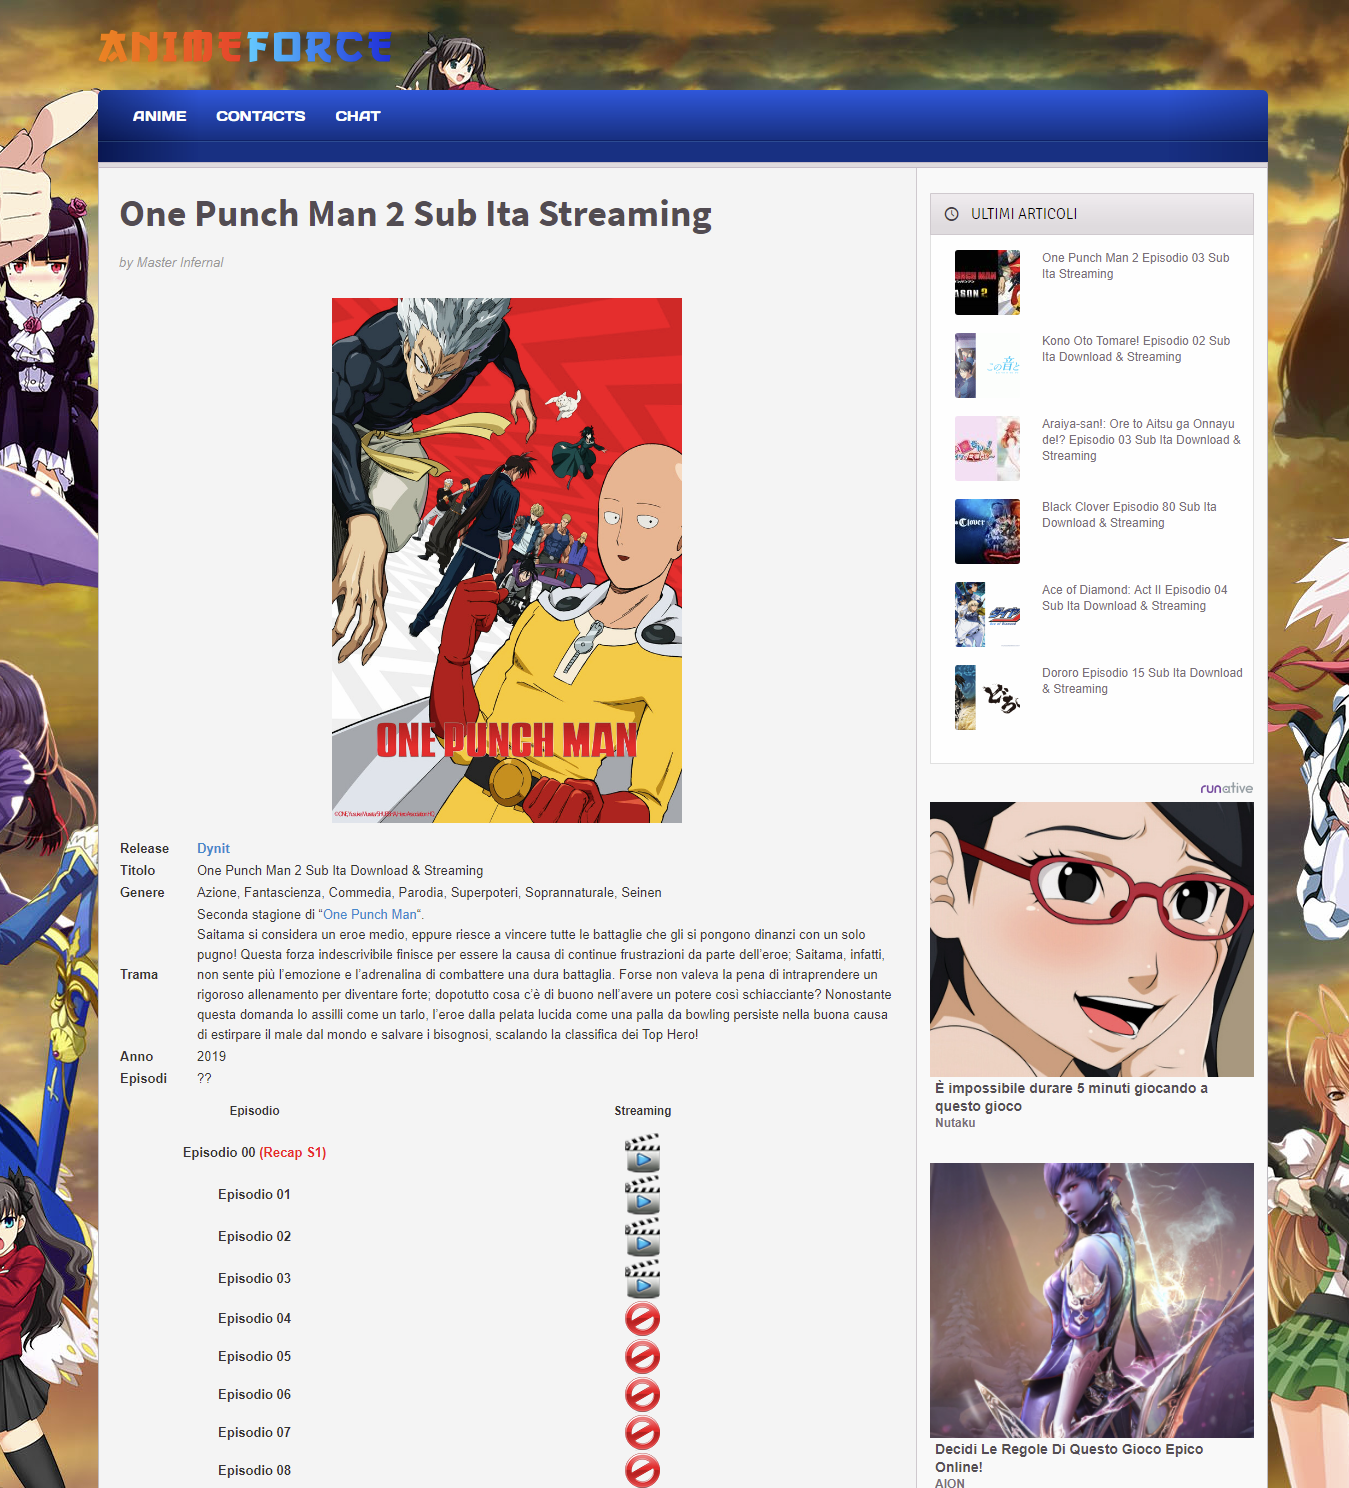
\includegraphics[width=0.5\textwidth]{img/Pag2_01.png}
	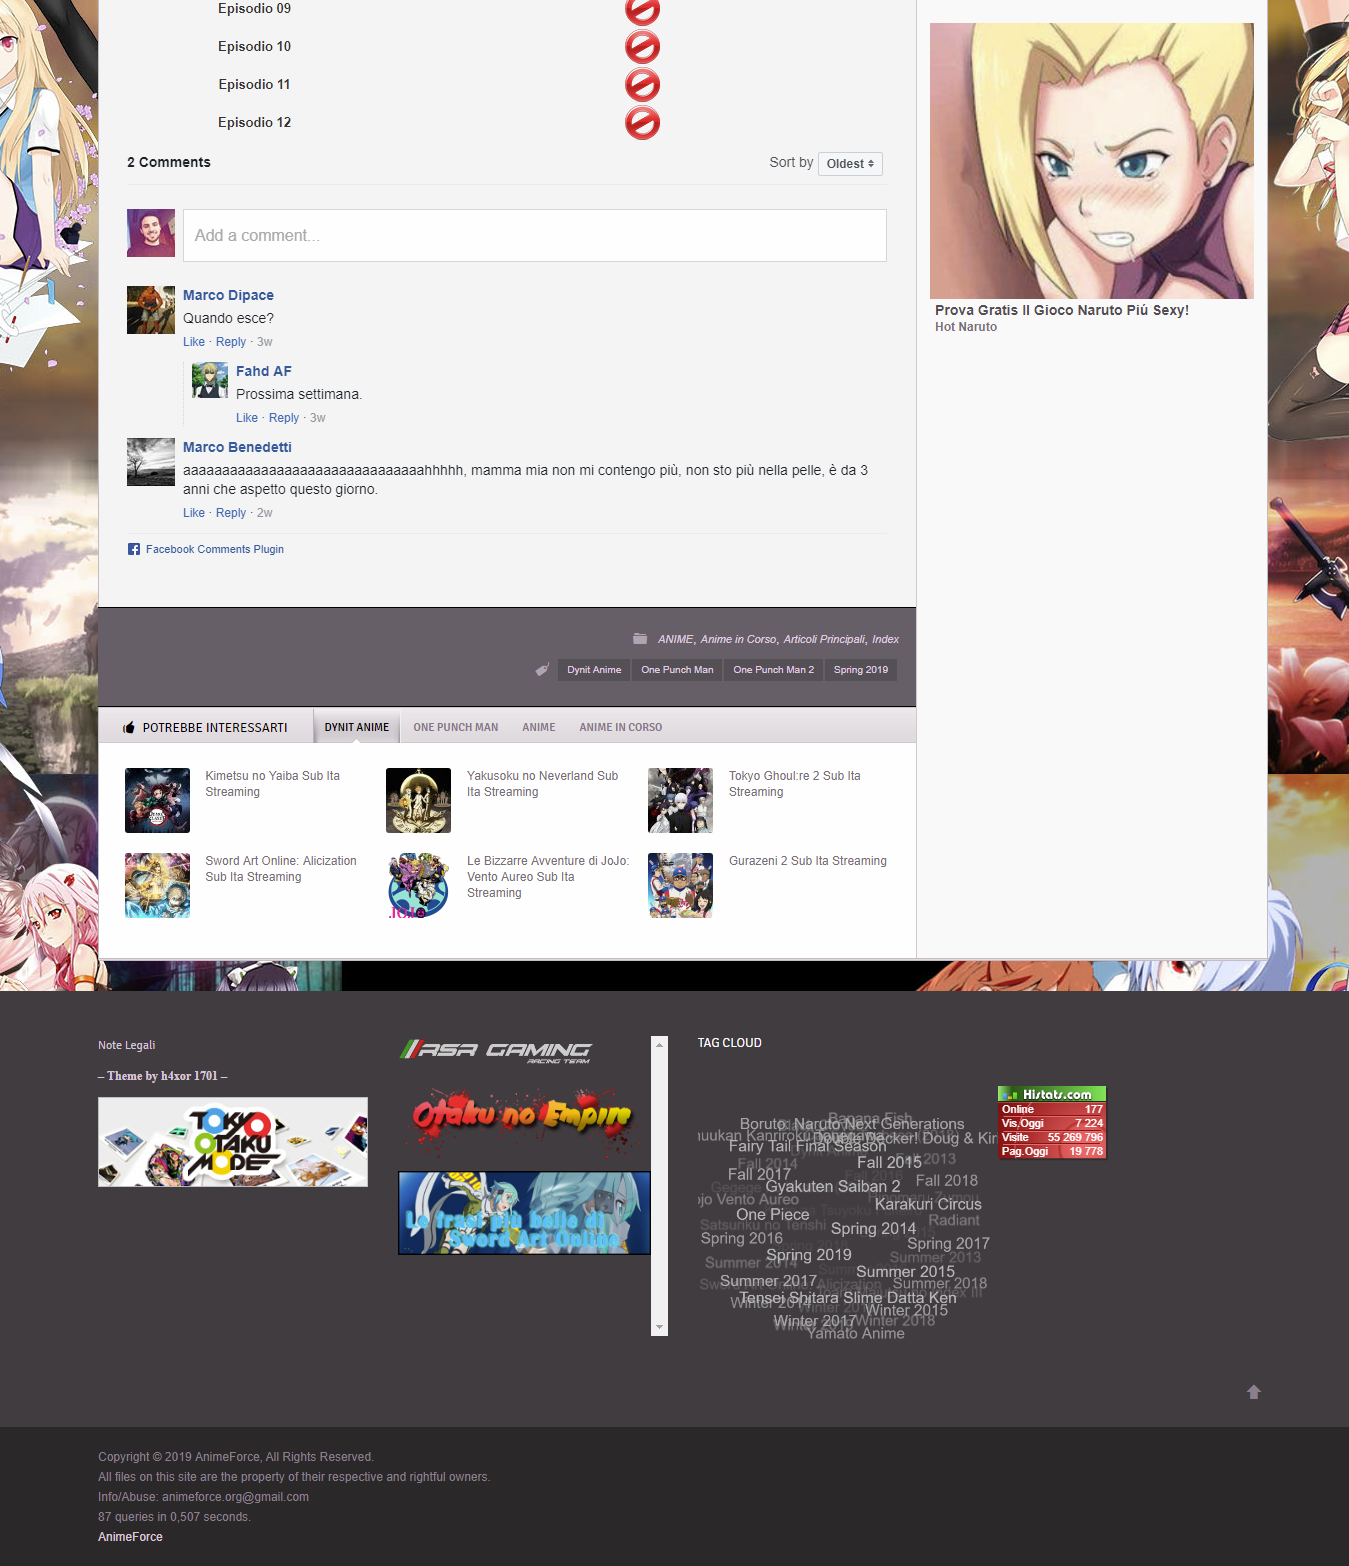
\includegraphics[width=0.5\textwidth]{img/Pag2_02.png}
	\caption{Altra pagina del sito: la parte iniziale e quella finale.} 
	\label{img7} 
\end{figure}

Nelle pagine interne risultano di fondamentale importanza le seguenti W: "Who", "Where" e "What". Per quanto riguarda il Who quanto è stato detto nella \hyperref[Navigazione]{Sezione \ref{Navigazione}} è esauriente. Sebbene non sia importante il "When", nelle pagine interne troviamo una novità: una sezione dedicata ai suggerimenti per i prossimi anime da guardare.\\ \\
In questa sezione ci concentriamo nei restanti assi informativi e dedichiamo anche una piccola attenzione allo stile della pagina.

\paragraph{Where} Una pecca generale del sito è legata al fatto che non esiste alcun aiuto alla creazione di una mappa mentale e questo è un'esempio ad hoc. La seguente pagina è raggiungibile (escludendo il deep-linking) solo attraverso i seguenti passaggi: 
\begin{enumerate}
	\item Selezionare la voce di menù anime;
	\item Scorrere con il mouse e selezionare la voce "Anime in corso" o "Lista anime A-Z";
	\newpage
	\item Selezionare la lettera con cui inizia il titolo dell'Anime o effettuare scoll verticale;
	\item Selezionare il link "One Punch Man 2". 
\end{enumerate}
Per raggiungere una pagina interna al sito senza sfruttare la "Ricerca" abbiamo impiegato 4 click di cui non verrà tenuta alcuna memoria. Il numero di click è limitato, ma la mappa è fondamentale per un sito.

\paragraph{What} Per quanto riguarda il "What", oltre al link alla homepage, possiamo individuare il primo vero contenuto della pagina: il titolo, un'immagine, release, il titolo, genere, trama, anno, numero di episodi, l'elenco di quest'ultimi con un link alla pagina dove poterli guardare in streaming, una sezione dedicata ai commenti ed infine dei suggerimenti.
A livello contenutistico, a mio parere, la pagina è adeguata sebbene sia da migliorare: la presenza di due volte del titolo e il numero di episodi inserito con "??" ad indicare non si conosce quanti saranno.

\subparagraph{Design} 
A livello di design è completamente errato e poco attrattivo per l'utente. Il team della pagina dovrebbe prendere in considerazione la possibilità di mettere immagini più piccole e affiancare ad una o più di esse le descrizioni. Inoltre pensare di tramutare le parole a fianco a "Genere" in eventuali tag per le ricerche.
Infine per la tabella dedicata agli episodi, potrebbero pensare a renderla dinamica ovvero presentare un numero di episodi (non tutti), poterli ordinare dal più recente a quello passato e viceversa (cosa già resa possibile vedi \hyperref[img7]{Figura \ref{img7}}) e poterli scorrere cliccando dei pulsanti.

